\documentclass[20pt, a0paper, portrait]{tikzposter}

  \usepackage[utf8]{inputenc}
  \usepackage[T1]{fontenc}
  \usepackage{textcomp}
  \usepackage{arev}
  \usepackage{arevmath}
  \usepackage{arevtext}
  \usepackage{graphicx}
  \usepackage{wrapfig}
  \usepackage{microtype}
  \usepackage{tikz}
  \usetikzlibrary{arrows.meta}
  
  % Bibliography
  \usepackage[backend=biber,
  bibencoding=utf8,
  bibstyle=numeric-comp,
  %style=verbose, %verbose-ibid,
  url=true, % include url in reference
  doi=true, % include doi in reference
  sorting=none, % sorting of citations
  %autocite=superscript, % autocite becomes superscript
  maxcitenames=1, % Max names displayed when citing in text
  maxbibnames=10, % Max number of names displayed in the bibliography
  giveninits=true % Use initials
  ]{biblatex}
  \addbibresource{citations.bib}

  \renewcommand*{\bibfont}{\footnotesize}
  \renewcommand*\familydefault{\sfdefault}
  
  \title{Failure Modes of Shafts}
  \author{Engineering Design \& Manufacture Group}
  \date{\today}
  \institute{University of Bath, UK}
  
  \usetheme{Default}
  \usecolorstyle[colorPalette=GreenGrayViolet]{Default}
  \useblockstyle{Default}
  \usetitlestyle{Filled}
    
  \begin{document}
  
  \maketitle
  
  \begin{columns}
    \column{0.5}
      \block[]{Introduction}{

        Shafts can fail in a number of ways such as:
        \vspace{1em}
        \begin{itemize}
          \item Overloading
          \item Fatigue
          \item Torsional fatigue
          \item Rotational loading
        \end{itemize}
        \vspace{1em}
        To understand the points at which a shaft will fail. One has to understand the stresses that are being applied to the shaft and relate this to the material properties of the shaft. This poster will take you through the steps to calculate the Principal Stresses in a shaft section.
  
      }
      \block[]{Direct Stress}{
        The first is the direct stress acting through the shafts cross-section. If the shaft diameter is not large enough then shaft will simply break as if one were creating a cross-section through the shaft. The Direct Stress is given by Equation~\ref{equ-direct-stress}.

        \begin{equation}
          \sigma_d = \frac{F}{A}
          \label{equ-direct-stress}
        \end{equation}

        However, it is very rare for a shaft to fail through Direct Stress through the shafts cross-section. It is more likely that a shaft will fail due to the combined bending, hoop and torsional stresses acting on the outer surface of the shaft, which can be resolved using Mohr's Circle~\autocite{clifford2012}.
      }
      \block[]{Mohr's Circle}{
        Taking a 2D element on the outer surface of the shaft, the bending, hoop and torsional stresses can be related as shown in Figure~\ref{fig-mohrs-circle}.

        \begin{tikzfigure}[2D Mohr's Circle]\label{fig-mohrs-circle}
          \center{}
          \begin{tikzpicture}[scale=5]
        
            \draw[] (0,0) -- (0,1) -- (1,1) -- (1,0) -- (0,0);
        
            \draw[->] (-0.1,0.5) -- (-0.4,0.5) node[left]{$\sigma_x$};
            \draw[->] (1.1,0.5) -- (1.4,0.5) node[right]{$\sigma_x$};
            \draw[->] (0.5,1.1) -- (0.5,1.4) node[above]{$\sigma_y$};
            \draw[->] (0.5,-0.1) -- (0.5,-0.4) node[below]{$\sigma_y$};
        
            \draw[{Straight Barb[left]}-] (0.0,-0.05) -- (1.0,-0.05) node[pos=0.0, below]{$\tau_{xy}$};
            \draw[-{Straight Barb[left]}] (0.0,1.05) -- (1.0,1.05) node[pos=1.0, above]{$\tau_{xy}$};
        
            \draw[{Straight Barb[right]}-] (-0.05,0.0) -- (-0.05,1.0) node[pos=0.0, left]{$\tau_{xy}$};
            \draw[-{Straight Barb[right]}] (1.05,0.0) -- (1.05,1.0) node[pos=1.0, right]{$\tau_{xy}$};
        
          \end{tikzpicture}
        \end{tikzfigure}

        Where:

        \begin{description}
          \itemsep0em
          \item[$\sigma_x$] Bending Stress
          \item[$\sigma_y$] Hoop Stress
          \item[$\tau_{xy}$] Torsional Stress
        \end{description}
      }
      \block[]{Bending Stress \(\sigma_x\)}{
        Bending stress is the Direct Stress in the direction of the axis of the shaft and is due to the bending moment. This can be calculated using Equation~\ref{equ-bending-stress}.

        \begin{equation}
          \sigma_{x} = \frac{My}{I}
          \label{equ-bending-stress}
        \end{equation}

        Where \(I\) is the Second Moment of Area:

        \begin{equation}
          I = \frac{\pi r^4}{4}
        \end{equation}
      }
      \block[]{Hoop Stress \(\sigma_y\)}{
        Hoop stress is the direct stress due to forces attempting to expand the shaft. This is becomes important when considering pressure vessels where the interior pressure of the gas or liquid is wanting to expand the vessel.

        \begin{equation}
          \sigma_y = \frac{F}{tl}
        \end{equation}

        Where:
        \begin{description}
          \itemsep0em
          \item[$F$] is the force exerted circumferentially on an area of the cylinder wall that has the following two lengths as sides:
          \item[$t$] is the radial thickness of the cylinder
          \item[$l$] is the axial length of the cylinder
        \end{description}
        
        In our cases, we can say that \(\sigma_y = 0\)
      }
    \column{0.5}
      \block[]{Torsional Stress \(\tau_{xy}\)}{
        Torsional stress is the shear stress due to torsion (twisting) and can by calculated using Equation~\ref{equ-torsional-stress}.

        \begin{equation}
          \tau_{xy} = \frac{Tr}{J}
          \label{equ-torsional-stress}
        \end{equation}

        Where \(J\) is the Polar Moment of Area:

        \begin{equation}
          J = \frac{\pi d^4}{32}
        \end{equation}
      }
      \block[]{Principal Stresses}{
        These stress depend upon the orientation of the element. If another element is taken, twisted through an angle \(\phi\), as shown in Figure, then the Direct Stresses are \(\sigma_x\) and \(\sigma_X\) and the shear stress is \(\tau_xy\) = \(\tau_XY\). And these are normally different from the first set of stresses in Figure~\ref{fig-rotated-mohrs-circle}.

        \begin{tikzfigure}[Mohr's circle rotated by \(\phi\)]\label{fig-rotated-mohrs-circle}
          \center{}
          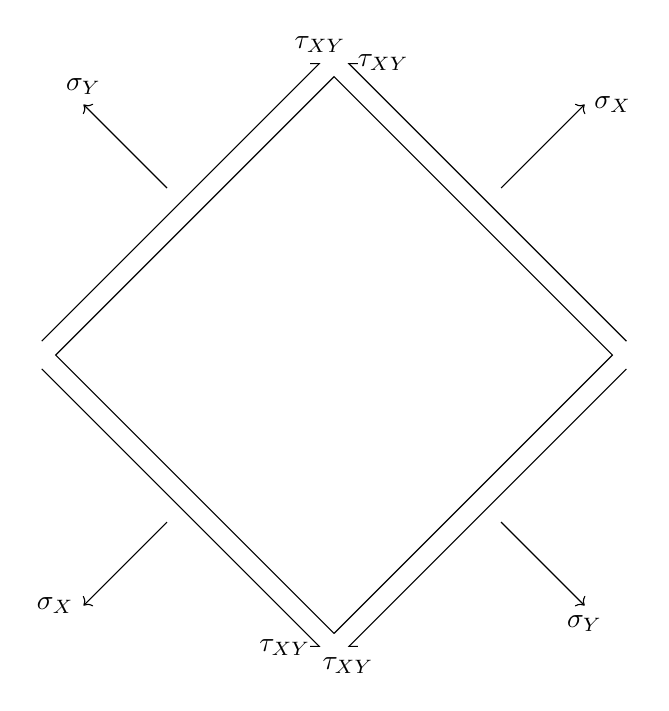
\begin{tikzpicture}[scale=5]

            \draw[rotate=45] (0,0) -- (0,1) -- (1,1) -- (1,0) -- (0,0);


            \draw[->, rotate=45] (-0.1,0.5) -- (-0.4,0.5) node[left]{$\sigma_X$};
            \draw[->, rotate=45] (1.1,0.5) -- (1.4,0.5) node[right]{$\sigma_X$};
            \draw[->, rotate=45] (0.5,1.1) -- (0.5,1.4) node[above]{$\sigma_Y$};
            \draw[->, rotate=45] (0.5,-0.1) -- (0.5,-0.4) node[below]{$\sigma_Y$};

            \draw[{Straight Barb[left]}-, rotate=45] (0.0,-0.05) -- (1.0,-0.05) node[pos=0.0, below]{$\tau_{XY}$};
            \draw[-{Straight Barb[left]}, rotate=45] (0.0,1.05) -- (1.0,1.05) node[pos=1.0, above]{$\tau_{XY}$};

            \draw[{Straight Barb[right]}-, rotate=45] (-0.05,0.0) -- (-0.05,1.0) node[pos=0.0, left]{$\tau_{XY}$};
            \draw[-{Straight Barb[right]}, rotate=45] (1.05,0.0) -- (1.05,1.0) node[pos=1.0, right]{$\tau_{XY}$};

          \end{tikzpicture}
        \end{tikzfigure}

        The two sets of stresses are related by formulae involving the sine and cosine of twice the angle, 2\(\phi\). Mohr's circle is a graphical way of representing these formulae. The construction of the circle is as follows and is shown in Figure~\ref{fig-m-circle}.

        \begin{enumerate}
          \item Draw the line AB between points with coordinates: \(\text{A} = (\sigma_x, -\tau_{xy}) \) and \(\text{B} = (\sigma_y, \tau_{xy}) \)
          \item Draw the circle with AB as diameter
        \end{enumerate}

        Then, to find the stresses related to the element rotated through angle \(\phi\), the diameter AB is rotated through angle \(2\phi\), giving diameter CD. The positions of C and D give the other stress with: \(\text{C} = (\sigma_X, -\tau_{XY}) \) and \(\text{D} = (\sigma_Y, \tau_{XY}) \).

        Mohr's circle shows there are two special cases. The first is when the diameter AB is rotated so that it becomes horizontal. The corresponding element undergoes no shear stress, but is subject to two direct stresses (in perpendicular directions) which are \(\sigma_1\) and \(\sigma_2\). These are the principal direct stress and represent the maximum and minimum values of direct stress in any direction.

        \begin{equation}
          \sigma_1 = \frac{1}{2}(\sigma_x+\sigma_y) + \sqrt{\left(\frac{1}{4}(\sigma_x-\sigma_y)^2\right)+\tau_{xy}^2}
        \end{equation}

        \begin{equation}
          \sigma_2 = \frac{1}{2}(\sigma_x+\sigma_y) - \sqrt{\left(\frac{1}{4}(\sigma_x-\sigma_y)^2\right)+\tau_{xy}^2}
        \end{equation}

        The second special case is when the diameter AB is rotated so that it becomes vertical in circle. The corresponding element sees the same direct stresses (in the two perpendicular directions) and a shear stress. From the figure, this common direct stress is the average of the principal stresses \(\frac{1}{2}(\sigma_1+\sigma_2)\). The shear stress is the largest possible shear stress in any direction, denoted (on the figure) by \(\tau_{\max}\).

        \begin{equation}
          \tau_{\max} = \sqrt{\left(\frac{1}{4}(\sigma_x-\sigma_y)^2\right)+\tau_{xy}^2}
        \end{equation}
      }
      \block[]{Limits}{
        In designing a component, there are limiting values placed on the direct and shear stresses (associated with any elements or directions). These may be based upon the yield tensile stress and the yield shear stress, or upon the ultimate tensile stress and ultimate shear stress.

        So there are two conditions to satisfy as follows.

        \begin{equation}
        |\sigma_1|,|\sigma_2| \leq \text{max\ allowable\ direct\ stress}
        \end{equation}

        \begin{equation}
        |\tau_{\max}| \leq \text{max\ allowable\ shear\ stress}
        \end{equation}
      }
      \block[]{References}{
        \printbibliography[heading=none]{}
      }
  \end{columns}
  
  \end{document}